\chapter{Proceso de aprendizaje}
\label{cap:AnexoF}

Este anexo documenta la evolución del proceso de entrenamiento del clasificador CIE-10, desde los primeros experimentos exploratorios hasta la configuración final desplegada en producción.

Durante las fases de exploración (Fases~1--4), los experimentos se realizaron sobre la tarea de \textbf{clasificación de capítulos CIE-10} (21 clases) como aproximación de primer nivel: el menor número de clases permite ciclos de entrenamiento cortos y resultados interpretables, y el ranking relativo de modelos se transfiere bien a la tarea real. El \textbf{clasificador final de producción} opera sobre los 1.767 \emph{block codes} de tres caracteres, proporcionando el código CIE-10 completo.

\section{Fases de exploración}

El desarrollo del clasificador atravesó varias fases que se corresponden con los \emph{notebooks} del directorio \texttt{bert-classifier/}:

\subsection{Fase 0: análisis de la arquitectura jerárquica}

El \emph{notebook} \texttt{0\_clasificador\_jerarquico\_Introducción.ipynb} exploró la hipótesis de entrenar clasificadores independientes por nivel jerárquico (capítulo → bloque → código específico). Esta aproximación se descartó por la propagación de errores entre niveles, tal como se justifica en el ADR-05 (\ref{cap:AnexoE}).

\subsection{Fase 1: RoBERTa-BSC base (evaluación)}

El \emph{notebook} \texttt{1\_clasificador\_jerarquico\_RoBERTa.ipynb} evaluó \texttt{PlanTL-GOB-ES/\allowbreak{}roberta-base-\allowbreak{}biomedical-clinical-es} como clasificador plano de primer nivel. El modelo se validó conceptualmente, pero no se llevó a producción por su ventana de contexto limitada a 512 tokens, que trunca la mayoría de los informes del corpus CodiEsp.

\subsection{Fase 2: IIC/RigoBERTa-2.0 (evaluación)}

El \emph{notebook} \texttt{2\_clasificador\_jerarquico\_RigoBERTa.ipynb} introdujo \texttt{IIC/RigoBERTa-2.0}~\cite{vacaserrano2022rigoberta}, versión de propósito general de RigoBERTa sobre arquitectura XLM-RoBERTa-large. Este modelo se evaluó conceptualmente como punto de partida previo a la variante clínica.

\subsection{Fase 3: mmBERT — primeros entrenamientos experimentales}

El \emph{notebook} \texttt{5\_clasificador\_jerarquico\_mmBert.ipynb} inició los experimentos con entrenamiento real sobre el corpus CodiEsp~\cite{miranda2020}. Se entrenaron 8 \emph{runs} con \texttt{jhu-clsp/mmBERT-base} sobre 809 códigos de bloque, con F1 micro entre 0{,}06 y 0{,}15.

\subsection{Fase 4: ModernBERT (evaluación)}

El \emph{notebook} \texttt{4\_clasificador\_jerarquico\_ModernBert.ipynb} evaluó la arquitectura ModernBERT~\cite{warner2024modernbert}, que obtuvo un F1-micro de 0{,}601 en pruebas de nivel~1. No se entrenó a fondo por restricciones de tiempo; queda identificado como candidato para iteraciones futuras (véase \ref{cap:AnexoA}).

\subsection{Fase 5: IIC/RigoBERTa-Clinical — entrenamiento intensivo}

A partir del \emph{run} 9 se adoptó \texttt{IIC/RigoBERTa-Clinical}~\cite{garciasubies2026rigobertaclinical} como modelo base. La fase 5 comprende 38 \emph{runs} en los que se ajustaron progresivamente los hiperparámetros: tasa de aprendizaje, congelación de capas, descongelación progresiva, \emph{dropout}, \emph{pos\_weight\_cap}, \emph{label smoothing} y umbral de clasificación. El F1 micro pasó de 0{,}32 (primer \emph{run}) a 0{,}489 (mejor \emph{run}).

\subsection{Fase 6: análisis de nivel 2}

El \emph{notebook} \texttt{7\_clasificador\_jerarquico\_analisis\_nivel\_2.ipynb} analizó la viabilidad de extender el clasificador plano a 4 caracteres (nivel de bloque específico). Se concluyó que las frecuencias de entrenamiento por código son insuficientes en el corpus actual para este nivel de especificidad.

\section{Evolución de los entrenamientos}

La Tabla~\ref{tab:training-evolution} recoge los hitos más relevantes de los 46 \emph{runs} registrados.

\begin{table}[h]
\centering
\caption{Hitos representativos del proceso de entrenamiento.}
\label{tab:training-evolution}
\begin{tabular}{clcrcc}
\hline
\textbf{Run} & \textbf{Modelo} & \textbf{Códigos} & \textbf{Épocas} & \textbf{F1 micro} & \textbf{Observación} \\
\hline
1  & mmBERT             & 809   & 19  & 0{,}061 & Línea base inicial \\
8  & mmBERT             & 809   & 20  & 0{,}150 & Mejor mmBERT \\
9  & RigoBERTa-Clinical & 809   & 20  & 0{,}320 & Cambio de modelo (+170\%) \\
19 & RigoBERTa-Clinical & 809   & 141 & 0{,}427 & Mejor con 809 códigos \\
21 & RigoBERTa-Clinical & 1767  & 79  & 0{,}327 & Expansión a espacio completo \\
27 & RigoBERTa-Clinical & 1767  & 60  & 0{,}470 & Introducción descongelación prog. \\
39 & RigoBERTa-Clinical & 1767  & 96  & 0{,}481 & Ajuste umbral y \emph{pos\_weight} \\
44 & RigoBERTa-Clinical & 1767  & 150 & 0{,}489 & Mejor F1 con umbral global \\
46 & RigoBERTa-Clinical & 1767  & 110 & 0{,}483 & Modelo desplegado en producción \\
\hline
\end{tabular}
\end{table}

\section{Comparativa de \emph{runs}}

La Figura~\ref{fig:all-trainings} muestra la comparativa de F1 micro y F1 macro de todos los \emph{runs}, a diferentes umbrales de clasificación (0{,}2, 0{,}3 y 0{,}5), junto con el número de épocas ejecutadas y la longitud máxima de secuencia empleada.

\begin{figure}[h]
\centering
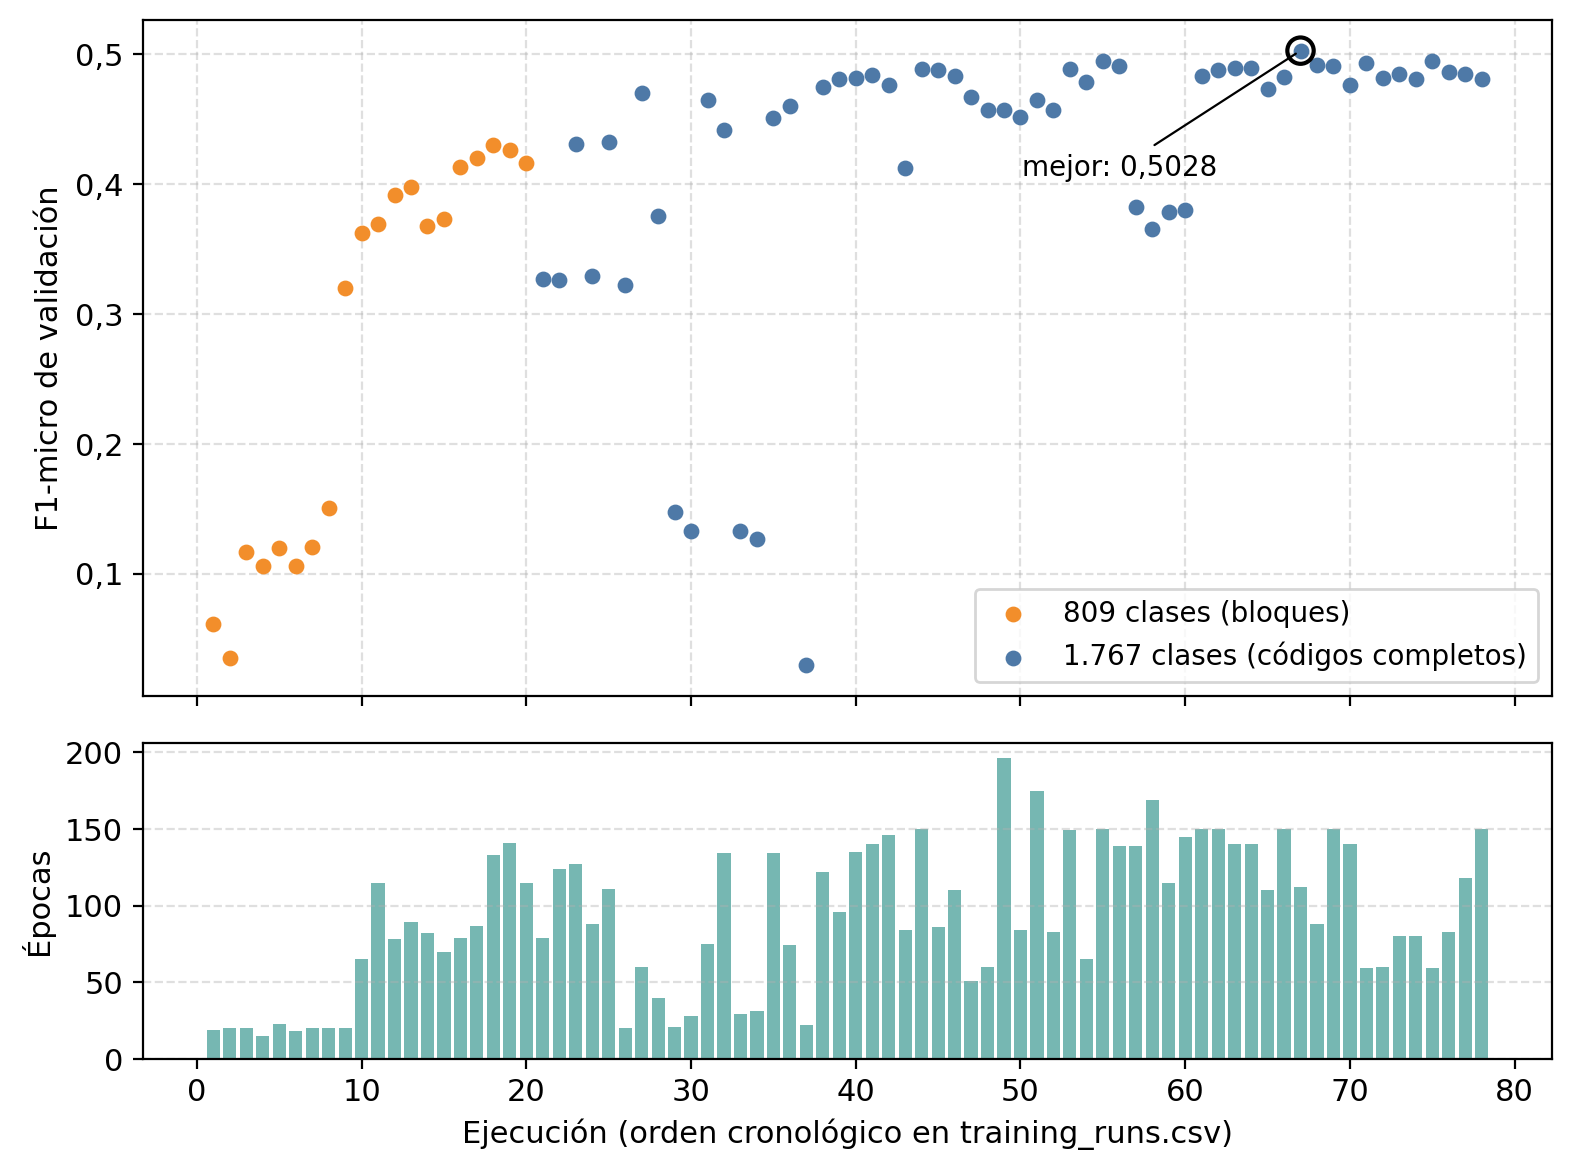
\includegraphics[width=\textwidth]{figs/all_trainings_graph}
\caption{Comparativa de F1 micro y F1 macro en todos los \emph{runs} del proceso de entrenamiento.}
\label{fig:all-trainings}
\end{figure}
